\newif\iffunny
\funnyfalse

\documentclass[xcolor={dvipsnames}]{beamer}
\usepackage{color, colortbl}
\usepackage[ngerman,english]{babel}
\usepackage[T1]{fontenc}
\usepackage{CJKutf8} %japanese
\usepackage{lmodern}
%\usepackage{subfigure}
\usepackage[compatibility=false]{caption}
\usepackage{subcaption}
\usepackage{tikz}
\usepackage{textgreek}
\usepackage{tabularx}
\usepackage{ragged2e}
\usepackage{adjustbox}
\usepackage{booktabs}
\usepackage{siunitx}
\usepackage{units}
\usepackage{appendixnumberbeamer}
\usepackage[absolute,overlay]{textpos} %for positioning the logos where I want

\usepackage{animate}
\usepackage{multimedia}
\usepackage{fixltx2e}
\usepackage{multicol}
\usepackage{comment}
\DeclareSIUnit\year{yr}

\mode<presentation>
{
  \usetheme{CambridgeUS}     
  \usecolortheme{lily} 
  \definecolor{beamer@violet}{rgb}{0.5,0.3,0.5} % changed this
  \setbeamercolor{structure}{fg=beamer@violet!70!cyan}
  \setbeamercolor{palette primary}{fg=black, bg=gray!30!white!50!cyan!20!}
  \setbeamercolor{palette secondary}{fg=black, bg=gray!30!white!30!cyan!40!}
  \setbeamercolor*{palette tertiary}{bg=gray!20!white!20!cyan!60!}
  
  \setbeamercolor{frametitle}{fg=cyan!60!white!40!,bg=cyan!80!black}
  \setbeamercolor{title}{fg=cyan!80!black}
  \setbeamercolor{normal text}{fg=black,bg=white}
  \setbeamercolor{alerted text}{fg=beamer@violet}
  \setbeamercolor{example text}{fg=beamer@violet!70!cyan}
  
  \usefonttheme{structureitalicserif} 
  \setbeamertemplate{navigation symbols}{}
  \setbeamertemplate{caption}[numbered]
}
\newcommand{\sidlogo}{
  \setlength{\TPHorizModule}{1pt}
  \setlength{\TPVertModule}{1pt}
   % textblock{}{x,y}: pos(x) = rightUpperCorner + (x * \TPHorizModule), pos(y) = leftUpperCorner - (y * \TPVertModule)
  \begin{textblock}{1}(323,12)
   \includegraphics[width=40pt,height=26pt]{figures/SiD.jpeg}
  \end{textblock}
  } 
\newcommand{\ilclogo}{
  \setlength{\TPHorizModule}{1pt}
  \setlength{\TPVertModule}{1pt}
   % textblock{}{x,y}: pos(x) = rightUpperCorner + (x * \TPHorizModule), pos(y) = leftUpperCorner - (y * \TPVertModule)
  \begin{textblock}{1}(323,12)
   \includegraphics[width=40pt,height=26pt]{figures/ILC.jpeg}
  \end{textblock}
} 
\newcommand{\ejadelogo}{
  \setlength{\TPHorizModule}{1pt}
  \setlength{\TPVertModule}{1pt}
   % textblock{}{x,y}: pos(x) = rightUpperCorner + (x * \TPHorizModule), pos(y) = leftUpperCorner - (y * \TPVertModule)
  \begin{textblock}{1}(323,12)
   \includegraphics[width=40pt,height=26pt]{figures/EJADE.jpeg}
  \end{textblock}
} 
\newcommand{\ATFlogo}{
  \setlength{\TPHorizModule}{1pt}
  \setlength{\TPVertModule}{1pt}
   % textblock{}{x,y}: pos(x) = rightUpperCorner + (x * \TPHorizModule), pos(y) = leftUpperCorner - (y * \TPVertModule)
  \begin{textblock}{1}(323,12)
   \includegraphics[width=40pt,height=26pt]{figures/ATF_logo.jpg}
  \end{textblock}
} 
\newcommand{\RHULlogo}{
  \setlength{\TPHorizModule}{1pt}
  \setlength{\TPVertModule}{1pt}
   % textblock{}{x,y}: pos(x) = rightUpperCorner + (x * \TPHorizModule), pos(y) = leftUpperCorner - (y * \TPVertModule)
  \begin{textblock}{1}(337,12)
   \includegraphics[width=25pt,height=26pt]{figures/rhul_logo.png}
  \end{textblock}
}
\newcommand{\flukalogo}{
  \setlength{\TPHorizModule}{1pt}
  \setlength{\TPVertModule}{1pt}
   % textblock{}{x,y}: pos(x) = rightUpperCorner + (x * \TPHorizModule), pos(y) = leftUpperCorner - (y * \TPVertModule)
  \begin{textblock}{1}(315,12)
   \includegraphics[width=60pt,height=26pt]{figures/fluka_logo.png}
  \end{textblock}
} 

\newcommand{\paper}{
  \setlength{\TPHorizModule}{1pt}
  \setlength{\TPVertModule}{1pt}
   % textblock{}{x,y}: pos(x) = rightUpperCorner + (x * \TPHorizModule), pos(y) = leftUpperCorner - (y * \TPVertModule)
  \begin{textblock}{65}(256,12)
  \centering
  \textblockcolour{SpringGreen}
  \vspace*{0.8mm}{arXiv:\\1609.07816v1}\vspace*{0.8mm}
  \end{textblock}
} 

\newcommand{\proceedigHelix}{
  \setlength{\TPHorizModule}{1pt}
  \setlength{\TPVertModule}{1pt}
   % textblock{}{x,y}: pos(x) = rightUpperCorner + (x * \TPHorizModule), pos(y) = leftUpperCorner - (y * \TPVertModule)
  \begin{textblock}{55}(266,12)
  \centering
  \textblockcolour{SpringGreen}
  \vspace*{0.8mm}{arXiv:\\1703.05737}\vspace*{0.8mm}
  \end{textblock}
} 

\newcommand{\proceedigBDS}{
  \setlength{\TPHorizModule}{1pt}
  \setlength{\TPVertModule}{1pt}
   % textblock{}{x,y}: pos(x) = rightUpperCorner + (x * \TPHorizModule), pos(y) = leftUpperCorner - (y * \TPVertModule)
  \begin{textblock}{55}(266,12)
  \centering
  \textblockcolour{SpringGreen}
  \vspace*{0.8mm}{arXiv:\\1703.05738}\vspace*{0.8mm}
  \end{textblock}
} 

\newcommand{\electron}{e$^-$}
\newcommand{\positron}{e$^+$}

\title[ILC \& Background Simulations]{\textbf{\LARGE The International Linear Collider \\ \large Background Simulations \& the Impact on SiD}}
\author[Anne Sch\"utz]{\underline{Anne Sch\"utz} \inst{1}, M. Stanitzki \inst {1}, J. Strube \inst{2}, B. Schumm \inst{3}, C. Milke \inst{3}, L. d`Hautuille \inst{3}, G. White \inst{4}, L. Keller \inst{4}, T. Barklow \inst{4}\\
\& SiD Optimization Group}

\institute[DESY]{\inst{1} DESY \inst{2} PNNL \inst{3} UCSC \inst{4} SLAC}
\date[May 1st 2017]{May 1st 2017\\\textbf{LC Vertex Detector Workshop 2017}}

\titlegraphic{
\includegraphics[height=1.2cm]{figures/DESY_Logo.png}\hspace*{1cm}~%
\includegraphics[height=1.2cm]{figures/PNNL_Logo.png}\hspace*{1cm}~%
\includegraphics[height=1.2cm]{figures/SiD.jpeg}\hspace*{1cm}~%
\includegraphics[height=1.2cm]{figures/UCSC_Logo.png}\hspace*{1cm}~%
\includegraphics[height=1.2cm]{figures/SLAC_Logo.png}
}

\begin{document}

{
\usebackgroundtemplate{
 \tikz\node[opacity=0.1]{\includegraphics[width=\paperwidth]{figures/Iwatecomics.jpg}};
 % \tikz\node[opacity=0.2]{\centering\includegraphics[height=\paperheight]{figures/Iwatecomics.jpg}};
 }
\begin{frame}
  \titlepage
\end{frame}
}

\begin{frame}{Table of contents}
%\begin{multicols}{2}
  \tableofcontents
%\end{multicols}
\end{frame}

\begingroup

\section{The SiD Detector}

\subsection{Overview}
\begin{frame}{SiD - Silicon Detector}
\sidlogo

\begin{columns}
\begin{column}{0.7\textwidth}
\alert{General Specifications}
\begin{itemize}
\item Height: $\sim$\SI{14}{\metre}, length:  $\sim$\SI{11}{\metre}
\item Weight: $\sim$\SI{10100}{\tonne}
\item Superconducting solenoid field: \SI{5}{\tesla}
\end{itemize}
\alert{Convincing design}
 \begin{itemize}
  \item Compact and robust
  \item Full silicon vertex detector and tracker
  \item Vertex detector:
  \begin{itemize}
   \item $<$\SI{5}{\micro\metre} resolution
   \item Momentum resolution $\sim$ 2-\SI{5e-5}{\per\giga\electronvolt}
   \item $\sim$ \SI{0.1}{\percent} X$_0$ per layer
  \item cos($\theta$)$\approx$0.984
  \end{itemize}

  \item Highly granular calorimetry optimized for Particle Flow (ECAL: radation length = 26 X$_0$, \\EM energy resolution = 0.17/$\sqrt{E}\bigoplus$1\%)
 \end{itemize}
\end{column}

\begin{column}{0.35\textwidth}
\begin{center}
\includegraphics[width=\textwidth]{figures/SiDpics.pdf}
\end{center}
\end{column}
\end{columns}

\end{frame}


\begin{frame}{SiD Detector Model} 
\sidlogo
\includegraphics[height=0.65\textheight]{figures/SiD_detector_model_2016.pdf}
\includegraphics[height=0.65\textheight]{figures/SiD_detector_model_Ausschnitt.pdf}\\
SiD detector model: Vertex/Tracker detector (red), ECAL (green), HCAL (pink), Muon system (blue)
\end{frame}


\AtBeginSubsection[] {
  \begin{frame}<beamer>
     \tableofcontents[currentsection,
     currentsubsection,
     %hideothersubsections,
     subsectionstyle=show/shaded/hide,
     subsubsectionstyle=show/show/hide]
  \end{frame}
}

\subsection{SiD Detector Variants}
\begin{frame}{Anti-DiD Field, L*, and the BeamCal ``plug''}
\sidlogo
\begin{columns}
 \begin{column}{0.7\textwidth}
 \alert{L* - Distance between IP and QD0}
  \begin{itemize}
  \item BeamCal attached to QD0 support structure
  \item L* change from 3.5\,m to 4.1\,m
  \item Resulting distance between IP and BeamCal: 3.265\,m
 \end{itemize}
 \alert{Anti-DiD Field}
 \begin{itemize}
  \item Directing pair background particles into the outgoing beam pipe
  \item Potentially suppress BeamCal backgrounds
 \end{itemize}
 \alert{BeamCal ``plug''}
  \begin{itemize}
  \item Region around beampipe holes in BeamCal
  \item Three proposed designs for the plug region:
  \begin{itemize}
   \item Instrumentation of the full plug region
   \item Wedge-cutout
   \item Circle-cutout
  \end{itemize}
 \end{itemize}  
 \end{column}
 \begin{column}{0.35\textwidth}
  \includegraphics[width=\textwidth]{figures/FwdPlusLayout.pdf}\\
  \vspace*{0.5cm}
  \includegraphics[width=\textwidth]{figures/AntiDiD-BeamCal.png}\\
  \vspace*{0.5cm}
  \includegraphics[width=0.33\textwidth]{figures/beamcal_plug.png}
  \includegraphics[width=0.33\textwidth]{figures/beamcal_wedge.png}
  \includegraphics[width=0.33\textwidth]{figures/beamcal_circle.png}
 \end{column}
\end{columns}

\end{frame}

%--------------------------------------------------------------

\section{Background Simulations \& the Impact on SiD}

\subsection{Background Sources \& Simulation Tools}
\begin{frame}{Background sources}
\ilclogo
\begin{block}{}
In order to minimize the effect of the background on the detectors and the measurements, the different background sources need to be modeled in great detail, also wrt a possible optimization of the Final-Focus layout.
\end{block}
\begin{columns}
 \begin{column}{0.65\textwidth}
 The main sources of background:
  \begin{itemize}
    \item Beam-beam interactions:
    \begin{itemize}
      \item Pair background
      \item Bhabha scattering
      \item \textgamma \textgamma $\rightarrow$ hadrons
    \end{itemize}
    \vspace*{0.3cm}
    \item Machine background:
    \begin{itemize}
      \item Muons from the Beam Delivery System
      \item Background from the Final-Focus system (beam halo collimators)
      \item Neutrons from the Beam Dumps
    \end{itemize}
  \end{itemize}
 \end{column}
 \begin{column}{0.4\textwidth}
 \begin{center}
 \includegraphics[width=0.33\textwidth]{figures/Bethe-Heitler.pdf}
 \includegraphics[width=0.33\textwidth]{figures/Breit-Wheeler.pdf}
 \includegraphics[width=0.33\textwidth]{figures/Landau-Lifshitz.pdf}\\
 \includegraphics[height=0.15\textheight]{figures/bhabha_scattering.pdf} 
 \includegraphics[height=0.15\textheight]{figures/gammagamma_hadrons.pdf}\\
 \vspace*{0.3cm}
 \includegraphics[width=0.8\textwidth]{figures/wall_shielding.png}  
 \end{center}
 \end{column}
\end{columns}
\end{frame}

\begin{frame}{Generator/Simulation tools}
The background is first modeled with different simulation tools:\\
\begin{itemize}
\item \alert{GuineaPig} (Generator of background events from beam-beam interactions)
\item \alert{BDSIM} (Geant4 based extension toolkit for beam line simulations)
\item \alert{FLUKA} (Fully integrated particle physics MonteCarlo simulation package)
\item \alert{MUCARLO} (Fortran tool to generate muons from the ILC Beam Delivery System)
\end{itemize}
The background events are then simulated in a \alert{full detector simulation} with a Geant4 toolkit.
\begin{figure}
	\begin{columns}
        \column{0.7\linewidth} \flushright
        \includegraphics[width=0.61\textwidth]{figures/Full_bunchcrossing_rhoz.png}
        \column{0.3\linewidth}
        {\small The inner detector part of SiD. WIRED4 event display of the pair background of one bunch crossing.}
      \end{columns}
\end{figure}
	
\end{frame}

\subsection{Background from High Cross Section ILC Processes}

\subsubsection{FCAL Occupancy}
\begin{frame}{Fractional loss of hits in the FCAL}
\sidlogo
\paper
  \begin{columns}
   \begin{column}{0.52\textwidth}
     \vspace*{0.5cm}\\
     With a \textbf{buffer depth of 4} in the current SiD electronics design, $\sim$ 0.3\% of all hits will be lost because of full buffers.\\
     \vspace*{1cm}
     \includegraphics[width=\textwidth]{figures/fig_radial_buffer_depth_all.png}
   \end{column}
   \begin{column}{0.52\textwidth}
     \includegraphics[width=0.95\textwidth]{figures/fig_buffer_depth.png}\\
     The fractional loss is clearly dependent on the radial position of the hit, so that this study suggests to \textbf{increase the number of buffers to 6} to reduce the fractional hit loss to below 10\textsuperscript{-3} at any radius.\\
    {\hfill \tiny Study done by B. Schumm and students at UCSC}
   \end{column}
  \end{columns}
\end{frame}

\subsubsection{BeamCal Reconstruction Efficiency}
\begin{frame}{BeamCal Reconstruction Efficiency}
\sidlogo
\paper
\begin{columns}
 \begin{column}{0.45\textwidth}
   The pair background is a specific brackground to the detection of individual high-energy \positron and \electron \,in the BeamCal.\\
   Especially at small radii, the \textbf{overall BeamCal reconstruction efficiency improves} with:
   \begin{itemize}
    \item an increase of L* from 3.5\,m (\textcolor{Blue}{blue}/\textcolor{Yellow}{yellow}) to 4.1\,m (\textcolor{Red}{red}/\textcolor{Green}{green})
    \item including the anti-DiD field (\textcolor{Green}{green} and \textcolor{Yellow}{yellow})
   \end{itemize}
 \end{column}
 \begin{column}{0.6\textwidth}
   \includegraphics[width=\textwidth]{figures/RadialEfficiency_total_160905.png}\\
    {\hfill \tiny Study done by B. Schumm and students at UCSC}
 \end{column}
\end{columns}
\begin{block}{}
 Dedicated physics studies need to be undertaken in order to fully assess the advantage of including the anti-DiD field.
\end{block}
\end{frame}


\subsubsection{Vertex Detector Occupancy}
\begin{frame}{Vertex Detector Occupancy}
\sidlogo
\paper
\begin{columns}
 \begin{column}{0.4\textwidth}
  Study of the \textbf{pair background occupancy in the VXD} in dependency of the SiD design choices:
 \end{column}
 \begin{column}{0.6\textwidth}
\adjustbox{max height=\dimexpr\textheight-5.5cm\relax,
           max width=\textwidth}{
\begin{tabular}{l|cc}
L* 4.1\,m & BeamCal ``plug'' design & anti-DiD \\ 
\hline
\textcolor{Red}{red}  & instrumented & $\times$\\
\textcolor{LimeGreen}{green}  & instrumented & \checkmark\\
\textcolor{Blue}{blue}  & circle cutout & $\times$\\
\textcolor{Turquoise}{turquoise} & wedge cutout & $\times$
\end{tabular}
}
 \end{column}
\end{columns}
   \includegraphics[width=0.51\textwidth]{figures/VradOccupancy_allGeoms_brl.png}\hspace*{0.1cm}
   \includegraphics[width=0.51\textwidth]{figures/VradOccupancy_allGeoms_ecp.png}\\
    {\hfill \tiny Study done by B. Schumm and students at UCSC}\\
  \textbf{Overall occupancies are small \& show little dependency on design.}
\end{frame}

\subsubsection{Vertex Detector Hit Time}
\begin{frame}{VXD - Pair background hit time}
\sidlogo
\paper
\textbf{Timing of the pair background wrt the bunch crossing}\\\vspace*{0.3cm}
\only<1>{
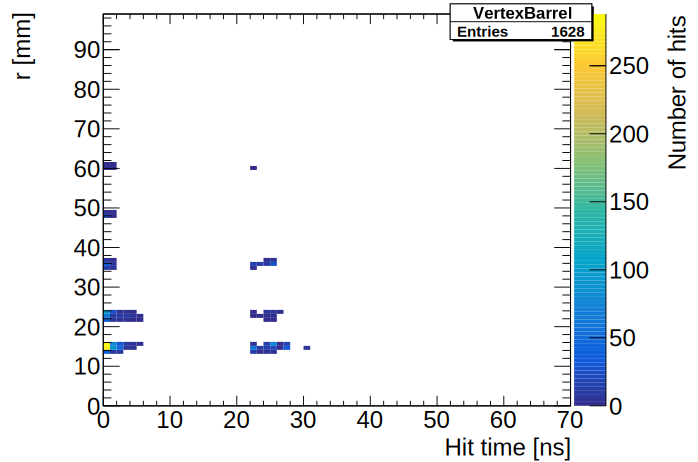
\includegraphics[width=0.5\textwidth]{figures/hittime_SiVertexBarrel.png}
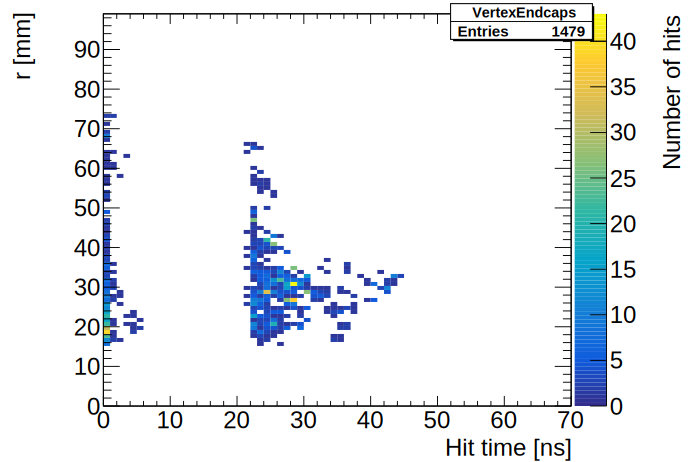
\includegraphics[width=0.5\textwidth]{figures/hittime_SiVertexEndcap.png}\\
}
\only<2>{
\includegraphics[width=0.5\textwidth]{figures/hittime_SiVertexBarrel_timeintervals.png}
\includegraphics[width=0.5\textwidth]{figures/hittime_SiVertexEndcap_timeintervals.png}\\
}
The vertex detector gets hits up to $\sim$ 50ns after the bunch crossing.\\
This is an opportunity to apply \textbf{time gates $\rightarrow$ background reduction!}
\end{frame}

\begin{frame}{Pair background - Particle origins}
\sidlogo
\paper
\only<1>{
\begin{center}
Particle origins of particles hitting the Vertex Detector in \textcolor{Red}{$[\unit[0]{ns};\unit[10]{ns}]$}
\includegraphics[width=0.7\textwidth]{figures/hitmaps_particleorigins_hittime_histo1_SiVertexEndcapSiVertexBarrel_SiDNote.pdf}
\end{center}
As expected, the pairs originate from the IP and the inner part of the detector.
}
\only<2>{
\begin{center}
Particle origins of particles hitting the vertex detector in \textcolor{Red}{$[\unit[10]{ns};\unit[20]{ns}]$}
\includegraphics[width=0.7\textwidth]{figures/hitmaps_particleorigins_hittime_histo2_SiVertexEndcapSiVertexBarrel_SiDNote.pdf}
\end{center}
The number of hits decreased, but there are still particles originating from the IP.
}
\only<3>{
\begin{center}
Particle origins of particles hitting the vertex detector in \textcolor{Red}{$[\unit[20]{ns};\unit[30]{ns}]$}
\includegraphics[width=0.7\textwidth]{figures/hitmaps_particleorigins_hittime_histo3_SiVertexEndcapSiVertexBarrel_SiDNote.pdf}
\end{center}
The pairs have travelled towards the detector endcaps and have backscattered there.
}
\only<4>{
\begin{center}
Particle origins of particles hitting the vertex detector in \textcolor{Red}{$[\unit[30]{ns};\unit[50]{ns}]$}
\includegraphics[width=0.7\textwidth]{figures/hitmaps_particleorigins_hittime_histo4_SiVertexEndcapSiVertexBarrel_SiDNote.pdf}
\end{center}
The particles still originate from the IP, the detector barrel and the endcaps.
}
\end{frame}

\begin{frame}{Pair background -  P\textsubscript{T}}
\sidlogo
Since their P\textsubscript{T} ranges between 0 and 2\,GeV, they form \textbf{helix tracks in the solenoid field}. The tracks extend to the inner detector layers, and leave up to several tens of hits.
\begin{center}
\includegraphics[width=0.7\textwidth]{figures/PT_hittime_primaries_SiVertexEndcapSiVertexBarrel.pdf}
\end{center}
\end{frame}

\begin{frame}{Pair background envelopes - 500GeV}
\proceedigHelix
Due to their momentum distributions, the envelopes of all pair background helixes have a characteristic shape:
   \includegraphics[width=0.52\textwidth]{figures/PairHelixes_500GeV_5T_10bunches_xz.png}\hspace*{0.1cm}
   \includegraphics[width=0.5\textwidth]{figures/HelixEnvelopes_Helix_tracks_xz_Helix_in_beampipe_10bunches_500GeV_5T.pdf}\\
The envelopes show that at any given point the beam pipe is 4mm away from 99.9\% of all pair particle tracks.
$\Rightarrow$ Possibility to \textbf{reduce the beam pipe \& vertex detector radius} by $\sim$2mm.\\
\textit{Study of possible \textbf{improvement in physics event reconstruction} needed, whilst looking at the increase in the background level at smaller radii.}
\end{frame}
%\begin{frame}{Pair background envelopes - 350GeV}
%\proceedigHelix
%   \includegraphics[width=0.51\textwidth]{figures/PairHelixes_350GeV_5T.png}\hspace*{0.1cm}
%   \includegraphics[width=0.51\textwidth]{figures/PairEnvelopes_350GeV_5T.png}
%\end{frame}
%\begin{frame}{Pair background envelopes - 250GeV}
%\proceedigHelix
%   \includegraphics[width=0.51\textwidth]{figures/PairHelixes_250GeV_5T.png}\hspace*{0.1cm}
%   \includegraphics[width=0.51\textwidth]{figures/PairEnvelopes_250GeV_5T.png}
%\end{frame}

\subsection{Muons from the BDS}

\begin{frame}{The BDS}
\proceedigBDS
\begin{center}
  \includegraphics[width=0.9\textwidth]{figures/BDS_electron_tunnel.pdf}
  \end{center}
The Beam Delivery System (BDS) contains the Final Focus System, and therefore focusses the beam on its way to the Interaction Point (IP).
\end{frame}
\begin{frame}{The BDS}
\proceedigBDS
\begin{center}
  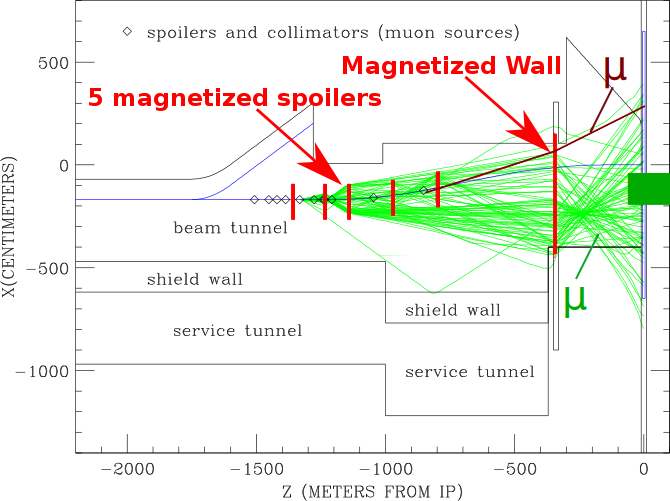
\includegraphics[width=0.7\textwidth]{figures/BDS_Tunnel_Spoilers+Wall.png}
\end{center}
Muons are created along the BDS, when the beam halo interacts with the beam line material.
\end{frame}

\begin{frame}{The Muon Spoilers}
\proceedigBDS
\begin{columns}
 \begin{column}{0.4\textwidth}
 The two suggested shielding scenarios:
  \begin{itemize}
   \item 5 Spoilers
   \begin{itemize}
    \item 70\,cm radius, 5\,m long
    \item magnetized iron
    \item at 5 locations along the BDS
   \end{itemize}
   \item 5 Spoilers + Wall
    \begin{itemize}
    \item 4\,m x 5\,m, 5\,m long
    \item magnetized iron
    \item close to the interaction region
   \end{itemize}
  \end{itemize}

 \end{column}
 \begin{column}{0.6\textwidth}
  \fbox{\includegraphics[width=\textwidth]{figures/Spoiler.png}}\\\vspace*{0.3cm}
  \fbox{\includegraphics[width=\textwidth]{figures/Muon_wall.pdf}}
 \end{column}
\end{columns} 
\end{frame}

\begin{frame}{WIRED4 event display - 5 Spoilers+Wall}
\sidlogo
\proceedigBDS
1 train's worth of muons ($\sim$ 515 muons) \textbf{from the positron line only}:
\begin{center}
\includegraphics[height=0.6\textheight]{figures/muons_positron_5spoilers_wall_515_xyview_croped.png}
{\tiny xy-view}
\includegraphics[height=0.6\textheight]{figures/muons_positron_5spoilers_wall_515_zyview_croped.png}
{\tiny zy-view}
\end{center}
Together with the muons from the e\textsuperscript{-} line, there will be \textbf{$\sim$ 900 muons per train in the '5 Spoilers + Wall' scenario}.
\end{frame}
\begin{frame}{WIRED4 event display - 5 Spoilers}
\sidlogo
\proceedigBDS
1 train's worth of muons ($\sim$ 2961 muons) \textbf{from the positron line only}:
\begin{center}
\includegraphics[height=0.6\textheight]{figures/muons_positron_5spoilers_2961_xyview_croped.png}
{\tiny xy-view}
\includegraphics[height=0.6\textheight]{figures/muons_positron_5spoilers_2961_zyview_croped.png}
{\tiny zy-view}
\end{center}
Together with the muons from the e\textsuperscript{-} line, there will be \textbf{$\sim$ 5600 muons per train in the '5 Spoilers' scenario}.\\
The spatial distribution is due to the tunnel shape and its shielding effects.
\end{frame}

\begin{frame}{Muon Occupancy in SiD ECAL endcaps}
\sidlogo
\proceedigBDS
\begin{center}
  \includegraphics[width=0.61\textwidth]{figures/EcalEndcap_DeadCells.png}
\end{center}
{\small A readout cell is ``dead'' when all buffers of the sensor are already filled. No more hits can be stored.}\\
The current SiD electronics design has a \textcolor{Green}{buffer depth of 4}, i.e. \textcolor{Blue}{10\textsuperscript{-6}} - \textcolor{Red}{10\textsuperscript{-4}} of all hits are dead in the ECAL endcaps.
\end{frame}

\begin{frame}{BDS Muon Study Conclusion}
\proceedigBDS
 With the shown results from the occupancy analysis of the muons from the current MUCARLO simulations, the \textbf{SiD group prefers to keep the magnetized wall} in order to keep the occupancy in the SiD detector as low as possible.
 \begin{columns}
  \begin{column}{0.4\textwidth}
    This will also allow access to the detector parking garage, since the wall represents a tertiary containment device against not only muons but also photons and neutrons from the machine background.
  \end{column}
  \begin{column}{0.6\textwidth}
    \includegraphics[width=\textwidth]{figures/wall_shielding.png}
  \end{column}
 \end{columns}
\end{frame}

\section{Further Ongoing Background Studies}

\subsection{Neutrons from the Beam Dumps}
{
\usebackgroundtemplate{
 \tikz\node[opacity=0.05]{\includegraphics[width=1.1\paperwidth]{figures/TB-0067-300-00-A_stamp.pdf}};
 % \tikz\node[opacity=0.2]{\centering\includegraphics[height=\paperheight]{figures/Iwatecomics.jpg}};
 }
\begin{frame}{FLUKA simulation of the ILC Beam Dump}
\flukalogo
The 16 MW beam is dumped into a water tank after collision.\\Neutrons ($\lesssim$\SI{e10}{\per\square\centi\metre\per\year}) are emitted that radiate the surroundings, and travel back towards the detectors.\\
\vspace*{0.1cm}
%Redoing the simulation studies that were done in 2007, when the design was not decided yet.
Concern about the safety and the functionallity of the beam dump design.
\begin{block}{Simulation step 1}
Simulating the neutrons from the beam dump with FLUKA, using the design drawings by B. Smith~\cite{Smith} to model the dump and the surrounding.
\end{block}

\begin{center}
\includegraphics[height=0.35\textheight]{figures/Front_view_BeamDump_Tomb.png}
\hspace*{0.2cm}
\includegraphics[height=0.35\textheight]{figures/Bird_view_BeamDump_Tomb.png}
\end{center}
\end{frame}

\begin{frame}{FLUKA simulation of the ILC Beam Dump}
\flukalogo
\begin{columns}
\begin{column}[c]{0.4\textwidth}
\includegraphics[height=0.45\textheight]{figures/FLUKA_quadrupole_model.png}\\
\small FLUKA simulation model of one of the ILC EXT lattice quadrupoles.
\end{column}
\begin{column}[c]{0.55\textwidth}
\begin{block}{Simulation step 2}
With Benno List (DESY): Python program to plug the real extraction line lattice into FLUKA.\\
Realistic simulation of the interaction between the neutrons and the lattice.
\end{block}
\begin{block}{Simulation step 3}
Simulating the neutrons reaching the interaction point in a full detector simulation.
\end{block}
\end{column}
\end{columns}
\end{frame}

\begin{frame}{Beam dump simulation goals}
 \flukalogo
 All goals of this study in an overview:
\begin{itemize}
 \item Simulating the neutron flux,
 \item the number of neutrons reaching the IP,
 \item the neutron occupancy in SiD,
 \item the dose of the beam dump surrounding,
 \item the influence of the water composition (amount of deuterium),
 \item the influence of the steel composition of the tank container,
 \item the amount of tritium produced in the water,
 \item the effect of the beam dump design.
\end{itemize}
\vspace*{0.5cm}
\rule{12cm}{.1pt}
\begin{thebibliography}{9}
\setbeamertemplate{bibliography item}[text]
\bibitem{Smith} B. Smith (Rutherford Lab), \emph{Design drawings 0-TB-0067-300-00-A, 0-TB-0067-210-00-A, 0-TB-0067-404-00-A}, Dec. 2006 - Jan. 2007
\end{thebibliography}
\end{frame}
}



\AtBeginSection[] {
  \begin{frame}<beamer>
     \tableofcontents[currentsection,
     currentsubsection,
     %hideothersubsections,
     subsectionstyle=show/shaded/hide,
     subsubsectionstyle=show/show/hide]
  \end{frame}
}

\section{Summary and Outlook}
\begin{frame}
\textit{Finished and ongoing background studies:}
 \begin{itemize} 
  \item Generation of \textbf{pair background GuineaPig files for 2 full ILC bunch trains} (available on the Grid)
  \item Study of the \textbf{timing and origin of pair background and backscattering particles} \textcolor{Green}{$\rightarrow$ possible reduction of background with time gates}
  \item \textbf{Pair helix envelopes} for 500, 350 and 250GeV ILC staging scenarios \textcolor{Green}{$\rightarrow$ suggested reducing the radius of beam pipe and vertex detector}
  \item Comparison between two different \textbf{muon shielding possibilies} and the muon occupancy in SiD \textcolor{Green}{$\rightarrow$ Spoilers + magnetized wall is prefered shielding option}
   \item \textbf{Modellation of the Beam Dump and the EXT line with FLUKA} in collaboration with Benno List (DESY). \textbf{FLUKA simulations of the neutron fluxes from the beam dump}, through the EXT line, towards the IP
  \item Implementing \textbf{PACMAN} (detector shield clamp) in the SiD geometry
 \end{itemize}
\end{frame}


\section*{The end}
{
\usebackgroundtemplate{
 \tikz\node[opacity=0.1]{\includegraphics[width=\paperwidth,resolution=200]{figures/ilc-Comic.png}};
 % \tikz\node[opacity=0.2]{\centering\includegraphics[height=\paperheight]{figures/Iwatecomics.jpg}};
 }
\begin{frame}
\ilclogo
\begin{center}
\vspace*{1cm}
\textcolor{RubineRed}{
	\LARGE Thanks!
}
\end{center}
\end{frame}
}

\section*{References}
\begin{thebibliography}{9}
\begin{frame}{References}
\bibitem{Paper} T. Barklow, et al. \emph{A Study of the Impact of High Cross Section ILC Processes on the SiD Detector Design}, arXiv:1609.07816
\bibitem{ProceedingBDS} A. Schuetz \emph{Pair Background Envelopes in the SiD Detector}, arXiv:1703.05737
\bibitem{ProceedingBDS} A. Schuetz, L. Keller, G. White \emph{A Study of the Impact of Muons from the Beam Delivery System on the SiD Performance}, arXiv:1703.05738
\bibitem{TDR} T. Behnke, et al.
\emph{The International Linear Collider - Technical Design Report}, 2013.
\bibitem{LHC TDR} \emph{LHC - Design Report}, \url{http://ab-div.web.cern.ch/ab-div/Publications/LHC-DesignReport.html}
\bibitem{IP beam parameters} ATLAS-CONF-2010-027. \emph{Characterization of Interaction-Point Beam Parameters Using the pp Event-Vertex Distribution Reconstructed in the ATLAS Detector at the LHC}, 2010. \url{http://cds.cern.ch/record/1277659/files/ATLAS-CONF-2010-027.pdf}
\end{frame}
\end{thebibliography}

\endgroup
%--------------------------------------------------------------------------------
\begingroup 
\appendix
\newif\iflattersubsect

\begin{frame}
\begin{center}
\LARGE Additional Material
\end{center}
  \tableofcontents
\end{frame}

\section{ILC}
\subsection{ILC parameters}

%------Definition for column color in table
\definecolor{Gray}{gray}{0.9}
\newcolumntype{g}{>{\columncolor{Gray}}r}
%-----------------------------------------
\begin{frame}{The beam parameters of the ILC}
\ilclogo

\begin{table}[]
\centering
\begin{tabularx}{\textwidth}{ll|rrrg}
\hline
& & \multicolumn{1}{>{\centering}p{1.5cm}}{\textbf{Baseline 500}} & \multicolumn{1}{>{\centering}p{1.5cm}}{\textbf{Lumi Upgrade}} & \multicolumn{1}{>{\centering}p{1.5cm}}{\textbf{TeV Upgrade}} & {\centering\textbf{LHC 25ns}} \\ 
\hline
\cline{1-6}
\hline
E$_{CM}$  &[\si{\GeV}] & 500  & 500  & \num{1000} & \num{14000}\\
n$_b$ & & \num{1312} & \num{2625} & \num{2450} &  \num{2808} \\
$\Delta t_b$ &[\si{\nano\second}] & 554  & 366   & 366 & 25 \\
N & & \num{2.0e10}  & \num{2.0e10}  & \num{1.74e10}  & \num{11.5e10}\\
q$_b$ &[\si{\nano\coulomb}] & 3.2  & 3.2  &  2.7 & 18.4 \\
$\sigma_x^*$ &[\si{\nano\metre}] & 474  & 474  &  481 & \num{16700}\\
$\sigma_y^*$ &[\si{\nano\metre}] & 5.9 &  5.9  &  2.8 & \num{16700}\\
$\sigma_z$ &[\si{\milli\metre}] & 0.3  &  0.3  &  0.25 & 0.755\\
L &[\si{\per\centi\metre\squared\per\second}] & \num{1.8e34} & \num{3.6e34} & \num{3.6e34} & \num{1.0e34}\\
\hline
\end{tabularx}
\end{table}
\end{frame}
\begin{frame}{ILC baseline parameters}
\ilclogo
\centering
	\includegraphics[width=\textwidth]{figures/ILCTDR-VOLUME_3-PART_II_ILCparameters.pdf}
\end{frame}
\begin{frame}{ILC parameters for the different upgrade stages}
\ilclogo
\centering
	\includegraphics[width=0.8\textwidth]{figures/ILCTDR-VOLUME_3-PART_II_ILCparametersUpgrades.pdf}
\end{frame}

\AtBeginSection[] {
  \begin{frame}<beamer>
     \tableofcontents[currentsection,
     currentsubsection,
     %hideothersubsections,
     subsectionstyle=show/show/hide]
  \end{frame}
}

\section{SiD - Subdetector Specifications}
\begin{frame}
 \begin{table}
\caption{Key parameters of the baseline SiD design, including the measurements of the subdetectors, and their readout cell dimensions. The given readout cell dimension are the pixelation cell sizes used for the full detector Geant4 simulation.}
\label{tab:KeyParametersSiD}
\begin{tabular}{>{\raggedright}p{1.8cm}>{\raggedright}p{2.4cm}>{\raggedright}p{2.2cm}>{\centering}p{1.2cm}>{\raggedright}p{1.2cm}>{\raggedright}p{1.2cm}>{\raggedright}p{1.2cm}}
\hline\hline
\textbf{SiD Barrel} & \textbf{Technology} & \textbf{Readout cell dimensions [mm$^2$]} & \textbf{Inner radius [cm]} & \textbf{Outer radius [cm]} & \textbf{z extent [cm]} \tabularnewline
\hline
Vertex detector & Silicon pixels & 0.05 x 0.05 & 1.4 & 6.0 & $\pm 6.25$ \tabularnewline
Tracker & Silicon strips & 0.05 x 0.05 & 21.7 & 122.1 & $\pm 152.2$ \tabularnewline
ECAL & Silicon pixels- W & 3.5 x 3.5 & 126.5 & 140.9 & $\pm 176.5$ \tabularnewline
HCAL & RPC - steel & 10 x 10 & 141.7 & 249.3 & $\pm 301.8$ \tabularnewline
Solenoid & 5 T SC & - & 259.1 & 339.2 & $\pm 298.3$ \tabularnewline
Flux return & Scintillator- steel & 30 x 30 & 340.2 & 604.2 & $\pm 303.3$ \tabularnewline
\hline
\end{tabular}
\end{table}
\end{frame}

\begin{frame}
 \begin{table}
\begin{tabular}{>{\raggedright}p{1.8cm}>{\raggedright}p{2.4cm}>{\raggedright}p{2.2cm}>{\centering}p{1.2cm}>{\raggedright}p{1.2cm}>{\raggedright}p{1.2cm}>{\raggedright}p{1.2cm}}
\hline\hline
\textbf{SiD Endcap} & \textbf{Technology} & \textbf{Readout cell dimensions [mm$^2$]} & \textbf{Inner z [cm]} & \textbf{Outer z [cm]} & \textbf{Outer radius [cm]} \tabularnewline
\hline
Vertex detector & Silicon pixels & 0.05 x 0.05 & 7.3 & 83.4 & 16.6 \tabularnewline
Tracker & Silicon strips & 0.05 x 0.05 & 77.0 & 164.3 & 125.5 \tabularnewline
ECAL & Silicon pixel- W & 3.5 x 3.5 & 165.7 & 180.0 & 125.0 \tabularnewline
HCAL & RPC - steel & 10 x 10 & 180.5 & 302.8 & 140.2 \tabularnewline
Flux return & Scintillator- steel & 30 x 30 & 303.3 & 567.3 & 604.2 \tabularnewline
LumiCal & Silicon- W & 3.5 x 3.5 & 155.7 & 169.55 &  20.0 \tabularnewline
BeamCal & Semicond.- W & 3.5 x 3.5 & 326.5 & 344 & 14.0 \tabularnewline
\hline\hline
\end{tabular}
\end{table}
\end{frame}

\section{Background from High Cross Section ILC Processes}
\subsection{FCAL Occupancy}
\begin{frame}{Occupancy in the FCAL}
  \begin{center}
     \includegraphics[width=0.7\textwidth]{figures/fig_raw_occupancy.png}
  \end{center}
  Number of hits per channel during a full ILC bunch train ($\sim$2600 bunch crossings).\\
  {\hfill \tiny Study done by B. Schumm and students at UCSC}
\end{frame}

\AtBeginSubsection[] {
  \begin{frame}<beamer>
     \tableofcontents[currentsection,
     currentsubsection,
     %hideothersubsections,
     subsectionstyle=show/shaded/hide,
     subsubsectionstyle=show/show/hide]
  \end{frame}
}

\subsection{Pair background timing}
\begin{frame}{Creation time of particles hitting the Vertex Detector}
\begin{columns}
 \begin{column}{0.5\textwidth}
Distribution of the time of creation (relative to the bunch crossing) of pair background particles (from 1312 bunches) that hit the endcaps of the VXD.
At the time of the bunch crossing about \num{1.6e6} particles are created (underflow bin).\\
 {\footnotesize The creation time is plotted for pair background particles hitting the vertex endcaps only. This is to avoid double counting of particles that would hit both, the barrel and the endcaps.}
 \end{column}
 \begin{column}{0.55\textwidth}
 \includegraphics[width=1\textwidth]{figures/creationtime_histo_SiVertexEndcap_SiDNote.pdf}
 \end{column}
\end{columns}
 %\adjustbox{max height=\dimexpr\textheight-5.5cm\relax,
%           max width=\textwidth}{
\begin{table}
\footnotesize
\begin{tabular}{>{\RaggedRight}p{1.8cm}>{\RaggedRight}p{1.9cm}>{\RaggedRight}p{1.7cm}>{\RaggedRight}p{2.4cm}>{\RaggedRight}p{2.3cm}}
Overall pairs & Primary pairs [\unit[0]{ns};\unit[11]{ns}] & Late pairs ]\unit[11]{ns};\unit[50]{ns}] & Out-of-time backscatter pairs ]\unit[50]{ns};\unit[554]{ns}] & Out-of-time backscatter pairs ]\unit[554]{ns};\unit[1000]{ns}]\\
\hline
$\sim$ \num{1.9e6} & 87.33\% & 12.38\% & 0.16\% &  0.029\% 
\end{tabular}
\end{table}
%}
\end{frame}

\begin{frame}{Momentum distribution particles hitting the Vertex Detector}
  \includegraphics[width=0.5\textwidth]{figures/momentum_histo_SiVertexBarrelSiVertexEndcap_SiDNote.pdf}
  \includegraphics[width=0.5\textwidth]{figures/transvmomentum_histo_SiVertexBarrelSiVertexEndcap_SiDNote}\\
  Distributions of the pair background particle momenta of pair background particles from 1312 bunches that will hit the barrel and the endcaps of the vertex detector.
  The plots show the histograms of the total and the transverse momenta of the particles hitting the vertex detector, in certain time intervals.
\end{frame}

\subsection{Pair background helixes}
\begin{frame}{Explanation of helix track calculations}
\proceedigHelix
 \begin{center}
  \includegraphics[width=0.65\textwidth]{figures/Helix_explanation.png}
\end{center}
\end{frame}

\section{Muons from the BDS}
\begin{frame}{The Muons in SiD - Spatial Distribution}
\proceedigBDS
 \includegraphics[width=0.9\textwidth]{figures/Explanation_Spatial_distribution_NEW.pdf}
\end{frame}

\begin{frame}{The Muon Occupancy in SiD}
\proceedigBDS
 \includegraphics[width=0.6\textwidth]{figures/Hits_in_SiD_subdetectors_MuonSpoilerStudy.pdf}
  \includegraphics[width=0.45\textwidth]{figures/Explanation_Hits_Subdetectors.pdf}\\
The number of hits in the different SiD subdetectors for both shielding scenarios (\textcolor{Red}{``5 Spoilers''} and \textcolor{Blue}{``5 Spoilers + Wall''}) is not evenly distributed.\\
The number of hits depends on the effective area of the subdetector system.
 \end{frame}
 
 \begin{frame}{Muon Occupancy in SiD HCAL endcaps}
 \proceedigBDS
  \includegraphics[width=0.53\textwidth]{figures/muon_occupancy_deadcells_all_layers_HcalBarrel.pdf}
  \includegraphics[width=0.53\textwidth]{figures/muon_occupancy_deadcells_all_layers_HcalEndcap.pdf}\\
The current SiD electronics design has a \textcolor{Green}{buffer depth of 4}:\\
$\sim$\textcolor{Blue}{1$\times$10\textsuperscript{-6}} - \textcolor{Red}{4$\times$10\textsuperscript{-6}} of all hits are dead in the \textbf{HCAL barrel}\\
$\sim$\textcolor{Blue}{2$\times$10\textsuperscript{-4}} - \textcolor{Red}{1$\times$10\textsuperscript{-3}} of all hits are dead in the \textbf{HCAL endcaps}
\end{frame}

\begin{frame}{Muon Occupancy in SiD Tracker endcaps}
\proceedigBDS
\begin{center}
  \includegraphics[width=0.65\textwidth]{figures/SiTrackerEndcap_DeadCells.png}
\end{center}
The current SiD electronics design has a \textcolor{Green}{buffer depth of 4}, i.e. \textcolor{Blue}{10\textsuperscript{-8}} - \textcolor{Red}{10\textsuperscript{-7}} of all hits are dead in the Tracker endcaps.
\end{frame}
 
\begin{frame}{The Muon Energy}
\proceedigBDS
\begin{center}
  \includegraphics[width=0.65\textwidth]{figures/muon_energy.pdf}
\end{center}
The energy distribution of the muons from the ``5 Spoilers + Wall'' scenario does not reach the same maximum energy. The muons are decelerated and stopped within the magnetized wall.
\end{frame}

\endgroup

\end{document}
